\documentclass{beamer}
    
\mode<presentation> {

\usetheme{default}

\defbeamertemplate{footline}{author and page number}{
\begin{beamercolorbox}[ht=2.5ex,dp=1ex,center]{title in head/foot}
    \usebeamerfont{title in head/foot}
    \inserttitle
\end{beamercolorbox}%
\begin{beamercolorbox}[ht=2.5ex,dp=1ex,center]{author in head/foot}
    \usebeamerfont{author in head/foot}
    \insertshortauthor \, \, \, \, \, \, \, \, \, \, \, \,
    \, \, \, \, \, \, \, \, \, \, \, \, \, \, \, \, \, \, 
    \, \, \, \, \, \, \, \, \, \, \, \, \, \, \, \, \, \, 
    \, \, \, \, \, \, \, \, \, \, \, \, \, \, \, \, \, \, 
    \, \, \, \, \, \, \, \, \, \, \, \, \, \, \, \, \, \, 
    \insertpagenumber\,/\,\insertpresentationendpage\kern1em\vskip2pt%
\end{beamercolorbox}

}
\setbeamertemplate{footline}[author and page number]{}
\setbeamertemplate{navigation symbols}{} 
}

\usepackage{graphicx} % Allows including images
\usepackage{booktabs} % Allows the use of \toprule, \midrule and \bottomrule in tables
\usepackage{hyperref}

\title[Bachelor's Thesis Presentation]{TinyFace: Extreme Edge Face Detection on Embedded Devices} % The short title appears at the bottom of every slide, the full title is only on the title page

\author{Teodor Fratiloiu} % Your name
\institute[Technical University of Munich] % Your institution as it will appear on the bottom of every slide, may be shorthand to save space
{
% Technical University of Munich \\ % Your institution for the title page
\medskip
% \textit{teodor.fratiloiu@tum.de} % Your email address
}
\date{September 23, 2020} % Date

\begin{document}

\begin{frame}
\titlepage % Print the title page as the first slide
\end{frame}

% SLIDES
%--------------------------------------

\begin{frame}{\textbf{Why} Do Machine Learning on Microcontrollers}
    \begin{itemize}
        \item MCU's are already widely deployed - what if we used them to run \textit{non-deterministic, non-algorithmic} apps
        \item Compared to ML devices with server-client architectures:
        \begin{itemize}
        \item Data Processing \& Filtering earlier on (right at \textit{metal} level)
        \item Better efficiency and privacy
        \item Less Network Bottlenecks  
        \end{itemize}
        \item Opens up completely new use scenarios (e.g. smarter consumer IoT, more versatile industrial controllers etc.)
    \end{itemize}
\end{frame}
\begin{frame}{\textbf{Goals} for TinyFace - This Project}
\begin{enumerate}
    \item Face Detection with Machine Learning
    \item High Accuracy (Usable for Real-World Applications)
    \item Deployable to MCU's \cite{tinyml_book}
    \begin{itemize}
        \item Very small model size (less than 1 MB)
        \item Low-Power means more efficient apps are \textit{necessary}
        \item Less abstraction, more hardware programming
    \end{itemize}
    \item Using TensorFlow Lite, our own datasets and custom ML-models with our own training routines
\end{enumerate}
\end{frame}

\begin{frame}
\frametitle{Overview}
\tableofcontents
\end{frame}

\section{1. The ML-Powered Face Detection Workflow}
\begin{frame}{1. The ML-Powered Face Detection Workflow}
    \vspace{1 cm}
    
\includegraphics[height = 1.5 cm]{images/workflow.png} \par
    \vspace{1 cm}
    This means we have a 4-Step (Loop) Process: \par
    \begin{enumerate}
        \item Generate Custom Datasets
        \item Read papers on different model architectures and implement them ourselves
        \item Train said models with own data, compare results
        \item Develop an app to evaluate real-world accuracy
    \end{enumerate}
\end{frame}

\section{2. Compiling and Processing Datasets} 
\begin{frame}{2. Compiling and Processing Datasets}
\begin{itemize}
    \item Wrote up an automated tool to generate our own data
    \begin{itemize}
        \item Can search and categorize images of actors online
        \item Can filter and process these images
        \item Outputs organized and labelled datasets, with images set to desired sizes and color-spaces (color, b/w)
    \end{itemize}
    \item Downloaded several datasets, from amongst those popular in research papers
    \begin{itemize}
        \item Labelled Faces in the Wild \cite{lfwild_site}
        \item Aligned Images \cite{alignedfaces_site}
        \item YT Faces \cite{ytfaces_site}
    \end{itemize}
\end{itemize}
\end{frame}
\begin{frame}{Dataset Sizes, Dimensions and Samples}
    \begin{figure}
        \centering
        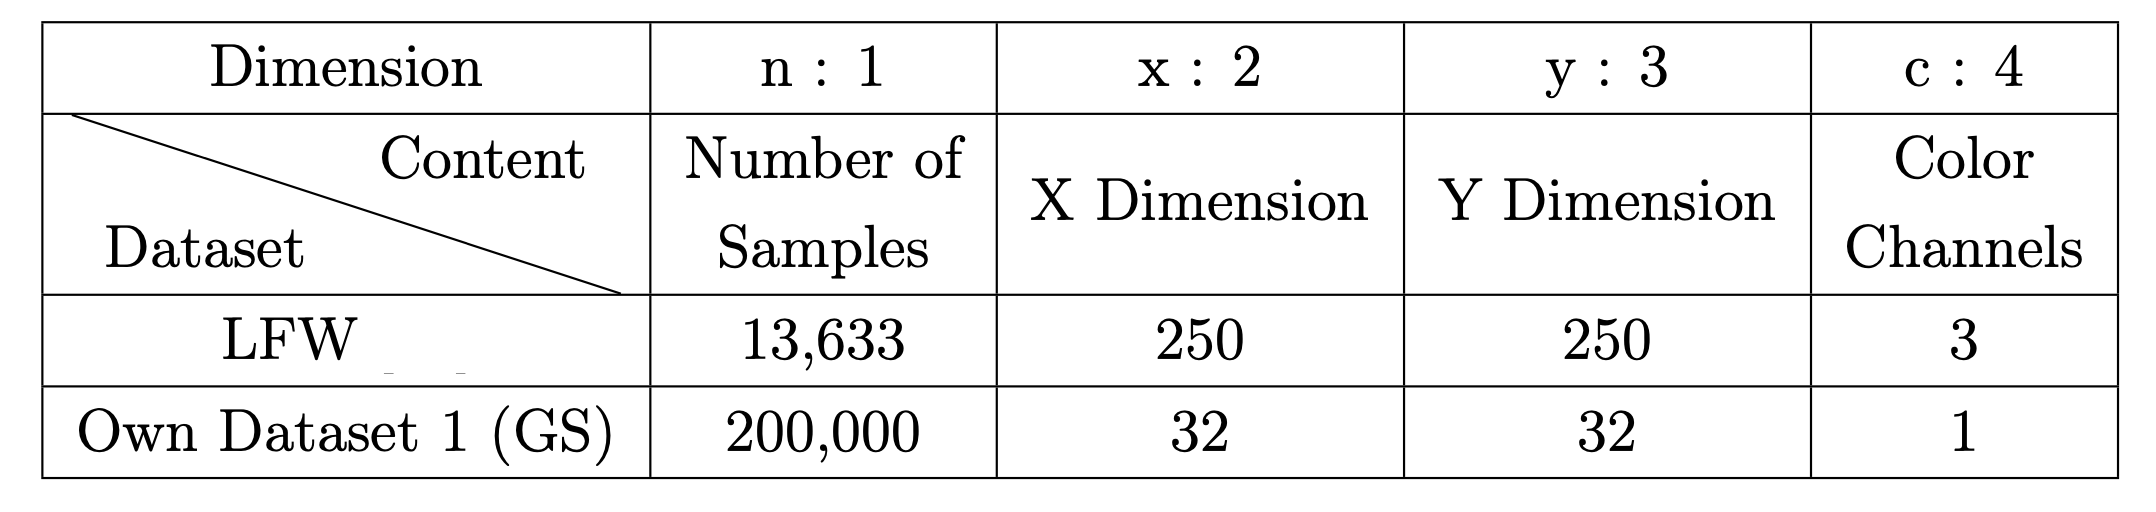
\includegraphics[width = 6 cm]{images/table 1.png}
        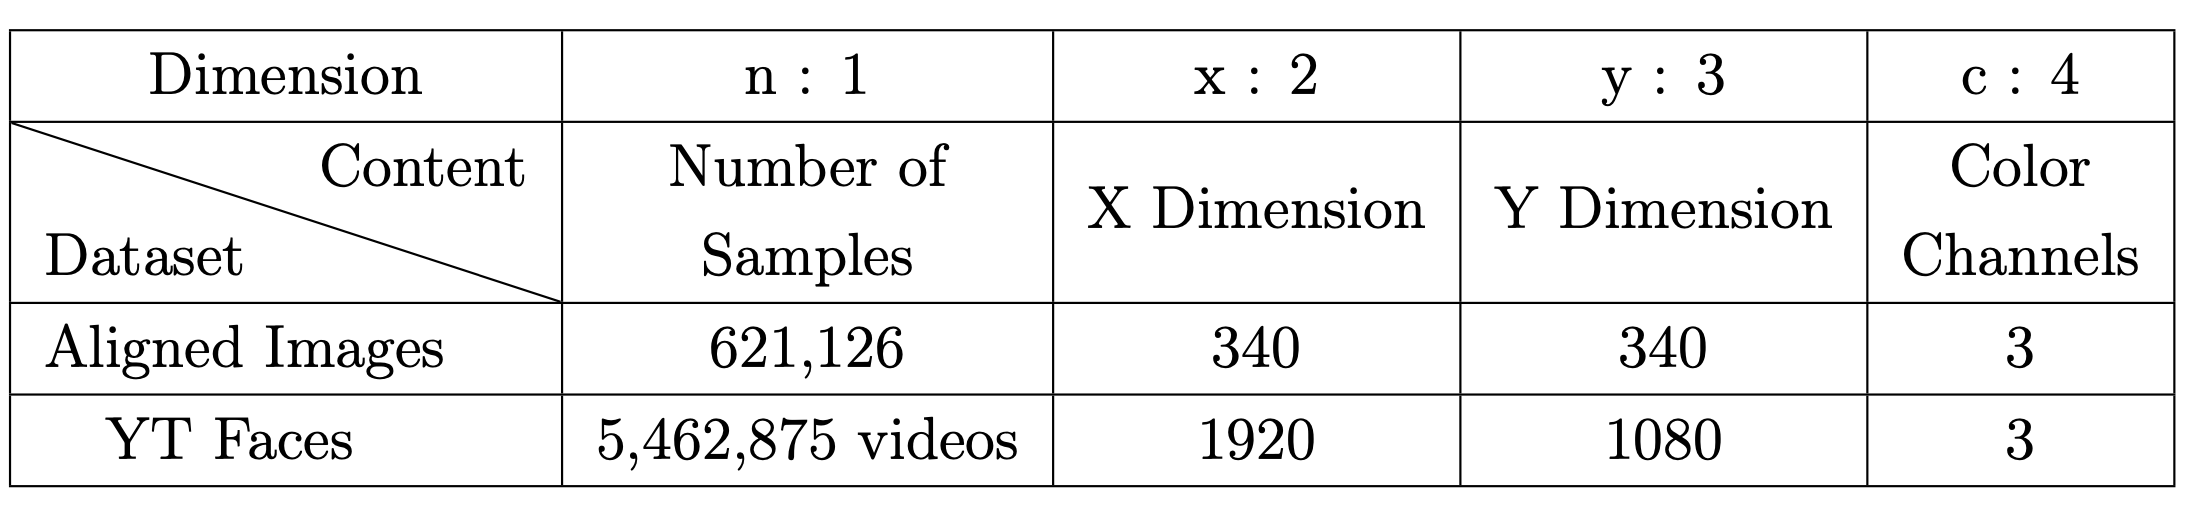
\includegraphics[width = 6 cm]{images/table 2.png}
        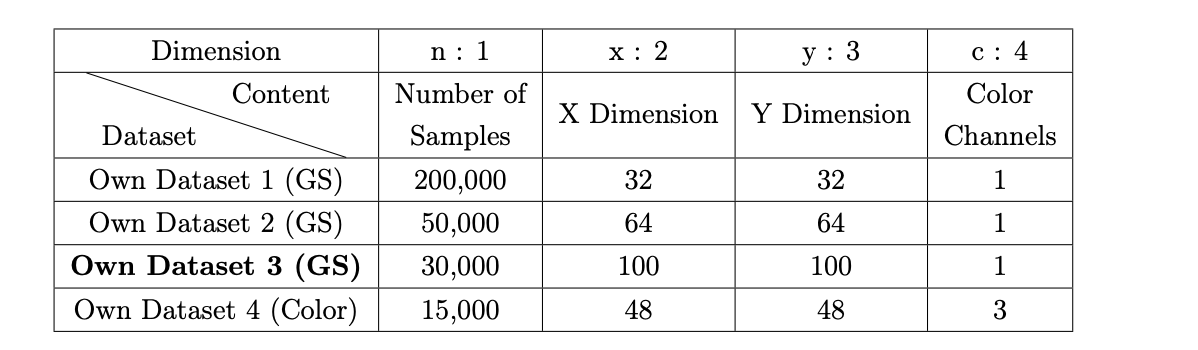
\includegraphics[width = 8 cm]{images/own dataset.png}
        % \caption{Sizes of Datasets}
        \label{fig:my_label}
    \end{figure}
    \begin{figure}
        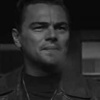
\includegraphics[width = 1.6 cm]{images/leo/3c5d0190660}\hfill
        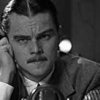
\includegraphics[width = 1.6 cm]{images/leo/3e3f6a53350}\hfill
        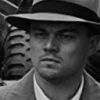
\includegraphics[width = 1.6 cm]{images/leo/3f4b0e0c760}\hfill
        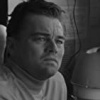
\includegraphics[width = 1.6 cm]{images/leo/4b605e33360}\hfill
        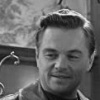
\includegraphics[width = 1.6 cm]{images/leo/24eb14f9da0}\hfill
        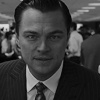
\includegraphics[width = 1.6 cm]{images/leo/188d3b34ff1}\hfill
        \caption{Sample Training Images with Randomized Padding Sides}
    \end{figure}
\end{frame}
\begin{frame}{What an Image Looks Like to The Model}
    \begin{figure}
    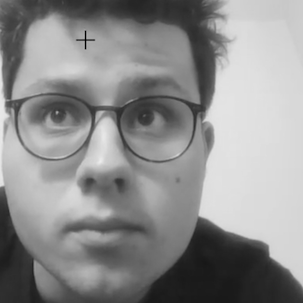
\includegraphics[width = 1.8 cm]{images/inference/63_35}\hfill
    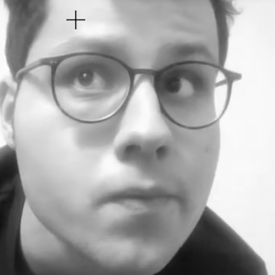
\includegraphics[width = 1.8 cm]{images/inference/48_51}\hfill
    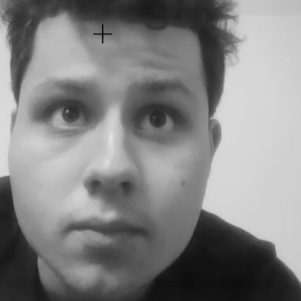
\includegraphics[width = 1.8 cm]{images/inference/61_38}\hfill
    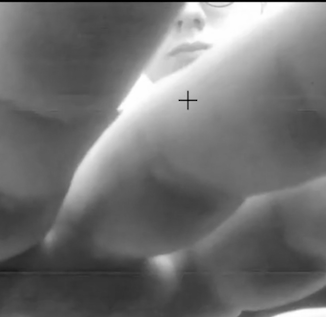
\includegraphics[width = 1.8 cm]{images/inference/41_58}\hfill
    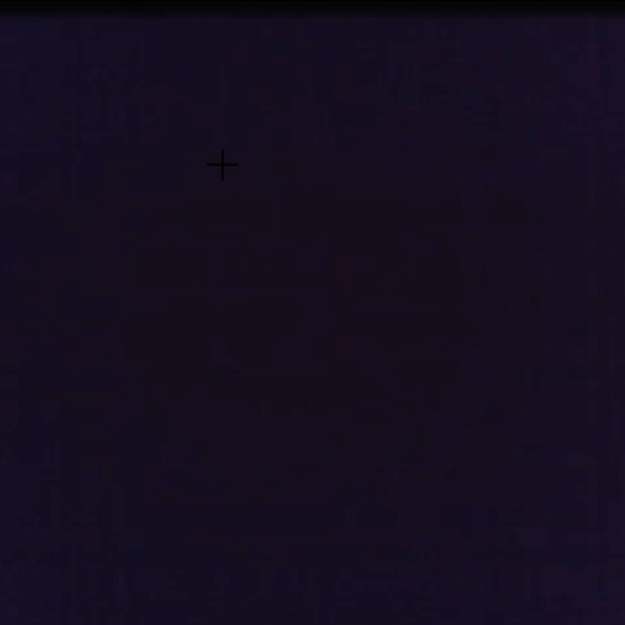
\includegraphics[width = 1.8 cm]{images/inference/37_62}\hfill
    \caption{Original images, as seen on webcam - cropped by hand to similar sizes for the sake of comparison with the images in the following figure and turned to black and white from color for consistency.}
    \label{webcam_orig}
\end{figure}

\begin{figure}
    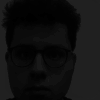
\includegraphics[width = 1.8 cm]{images/inference/frame_0}\hfill
    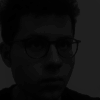
\includegraphics[width = 1.8 cm]{images/inference/frame_1}\hfill
    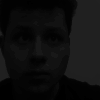
\includegraphics[width = 1.8 cm]{images/inference/frame_3}\hfill
    
\includegraphics[width = 1.8 cm]{images/inference/frame_4}\hfill
    
\includegraphics[width = 1.8 cm]{images/inference/frame_5}\hfill
    \caption{What the interpreter actually \textit{"sees"}. The images have sides of 100*100 pixels, their dynamic range has been downsampled to a value between 0 and 9 grayscale.}
    \label{interpreter_eyes}
\end{figure}
\end{frame}

\section{3. Implementing and Training ML Models} 
\begin{frame}{3. Implementing and Training ML Models}
        \begin{figure}
        \centering
        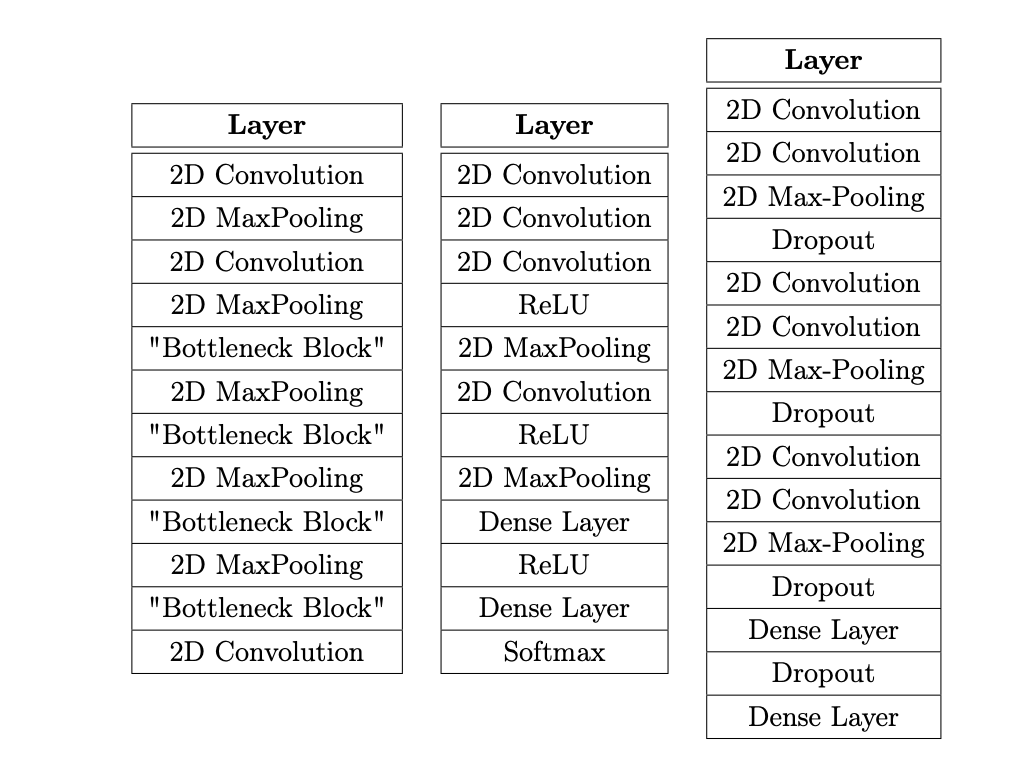
\includegraphics[width = 8 cm]{images/other_models.png}
        \caption{Architectures of Some Implemented Models, from Literature: DarkNet \cite{tiny_darknet}, LeNet \cite{lenet_paper}, VGG \cite{vgg_paper}} 
        \label{fig:model_sizes_trained}
    \end{figure}
\end{frame}
\begin{frame}{SqueezeNet Model Architecture}
        \begin{figure}
        \centering
        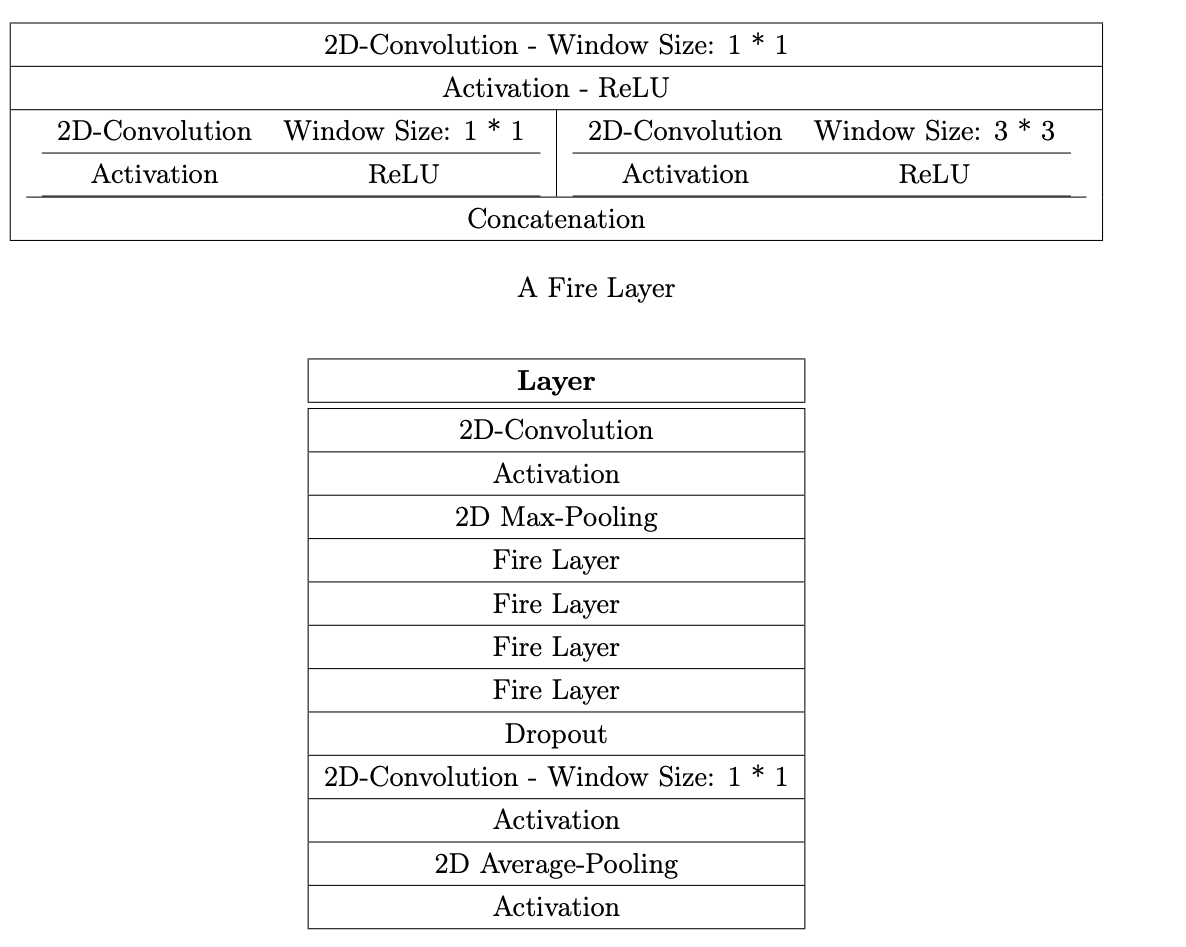
\includegraphics[width = 8 cm]{images/squeezenet_arch.png}
        \label{fig:model_sizes_trained}
    \end{figure}
\end{frame}
\begin{frame}{Implemented Models and their respective sizes}
    \begin{figure}
        \centering
        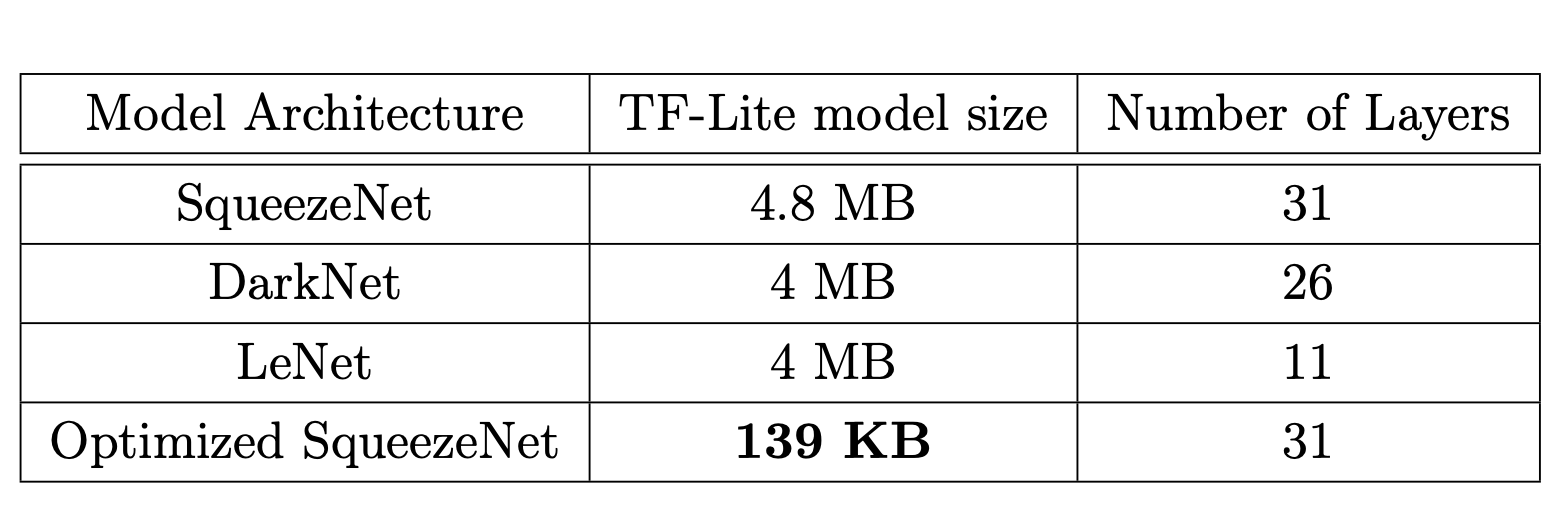
\includegraphics[width = 8 cm]{images/models_sizes.png}
        \caption{Final Sizes of some trained models}
        \label{fig:model_sizes_trained}
    \end{figure}
\end{frame}
\begin{frame}{Trained and Quantized SqueezeNet}
    \begin{figure}[!tbp]
        \subfloat{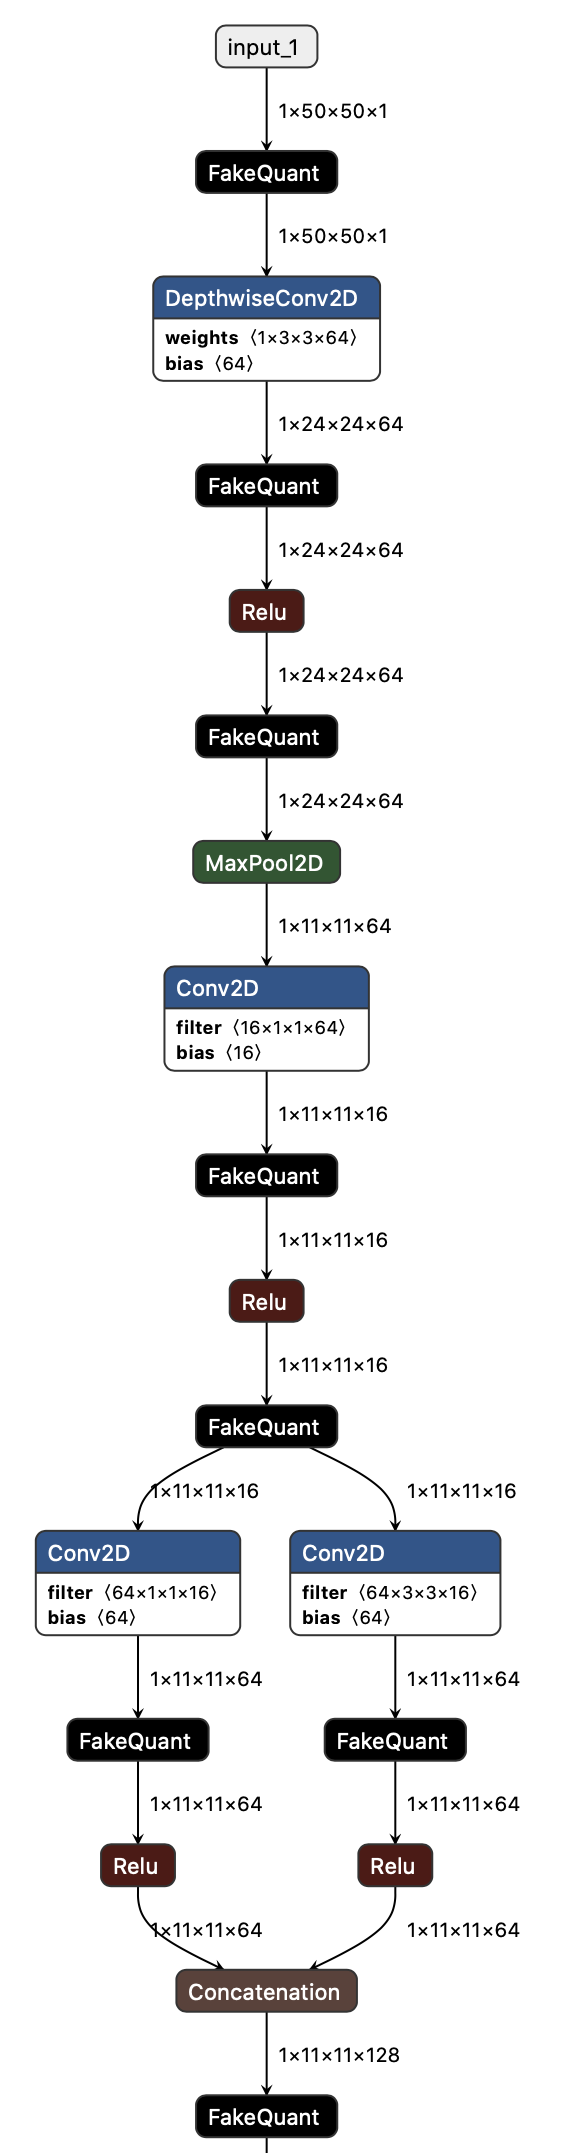
\includegraphics[height = 7.6 cm]{images/netron_sqnet_1.png}
        \label{fig:f1}}
        \subfloat{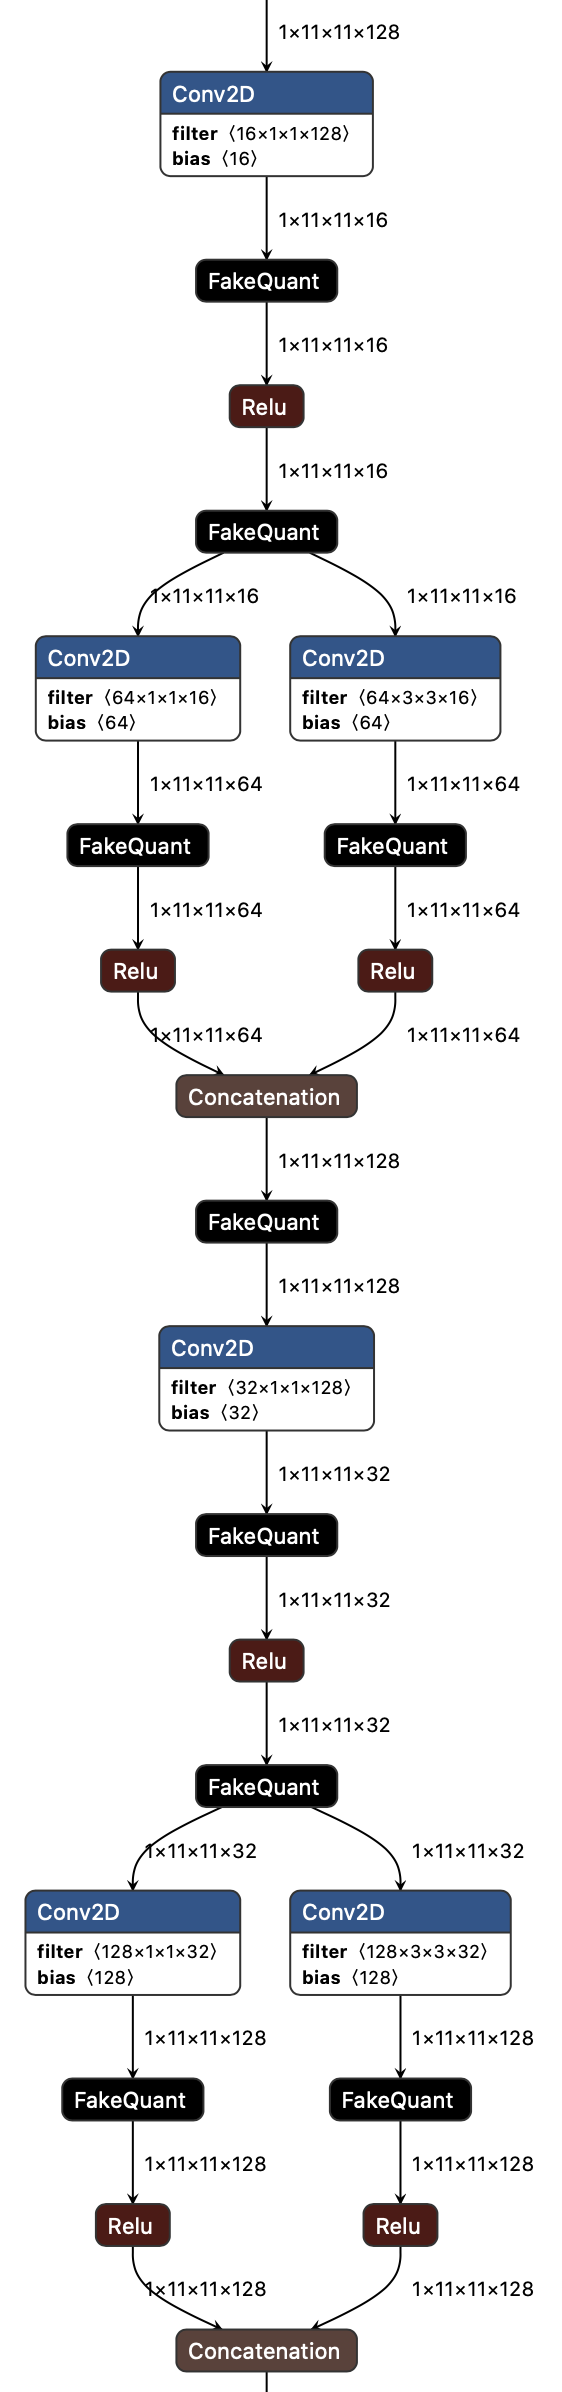
\includegraphics[height = 7.6 cm]{images/netron_sqnet_2.png}
        \label{fig:f2}}
        \subfloat{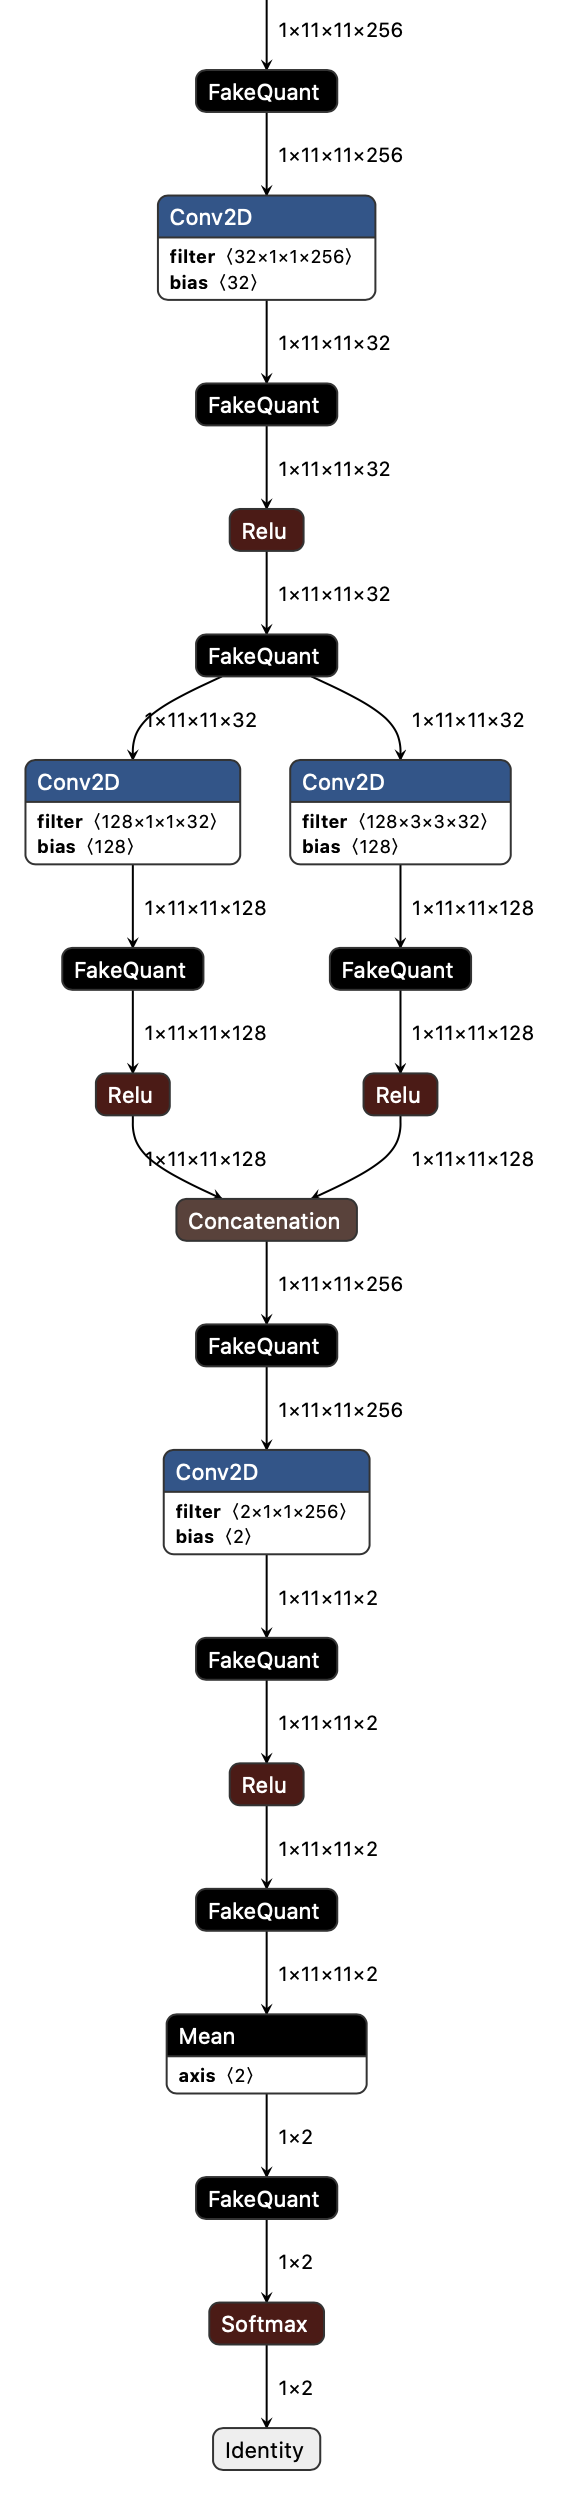
\includegraphics[height = 7.6 cm]{images/netron_sqnet_3.png}
        \label{fig:f3}}
        % \caption{Expanded view of trained and quantized Squeezenet (image was divided}
        \label{netron_sqnet}
    \end{figure}
\end{frame}
\begin{frame}{Training Performance of Squeezenet with Own Dataset}
    \begin{figure}[!tbp]
        \subfloat{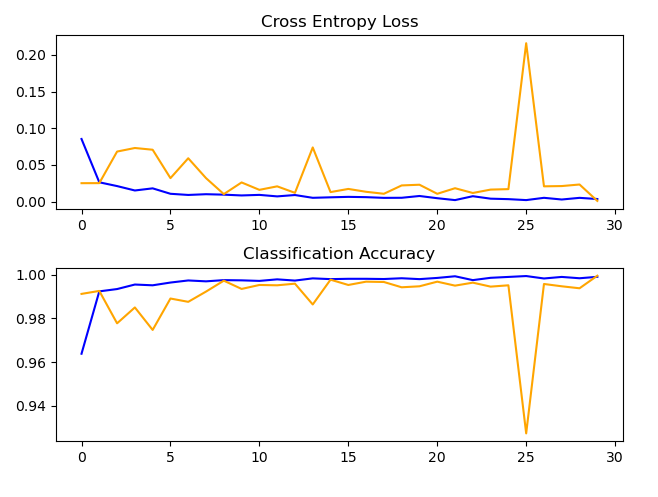
\includegraphics[height = 3.8 cm]{images/squeezenet_30ep_10bat_lfw_tfl.png}
        \label{fig:f1}}
        \subfloat{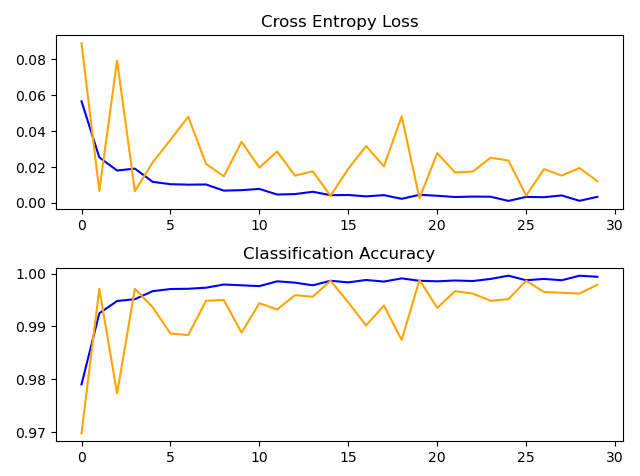
\includegraphics[height = 3.8 cm]{images/squeezenet_30ep_10bat_lfw_full.png}
        \label{fig:f2}}
        % \caption{Expanded view of trained and quantized Squeezenet (image was divided}
        \label{netron_sqnet}
    \end{figure}
\end{frame}


\section{4. TinyFace Evaluation Demo} 
\begin{frame}{4. TinyFace Evaluation Demo}
Properties of Used Model for Inference:
\begin{itemize}
    \item 5 Training Epochs
    \item A Batch Size of 32 Samples
    \item A 75\%-25\% Divide between Training and Test Data
    \item A Dropout Rate of 10\%
\end{itemize}
\end{frame}
\begin{frame}{Training Performance of Said Model}
    \begin{figure}[!tbp]
        \centering
        \subfloat{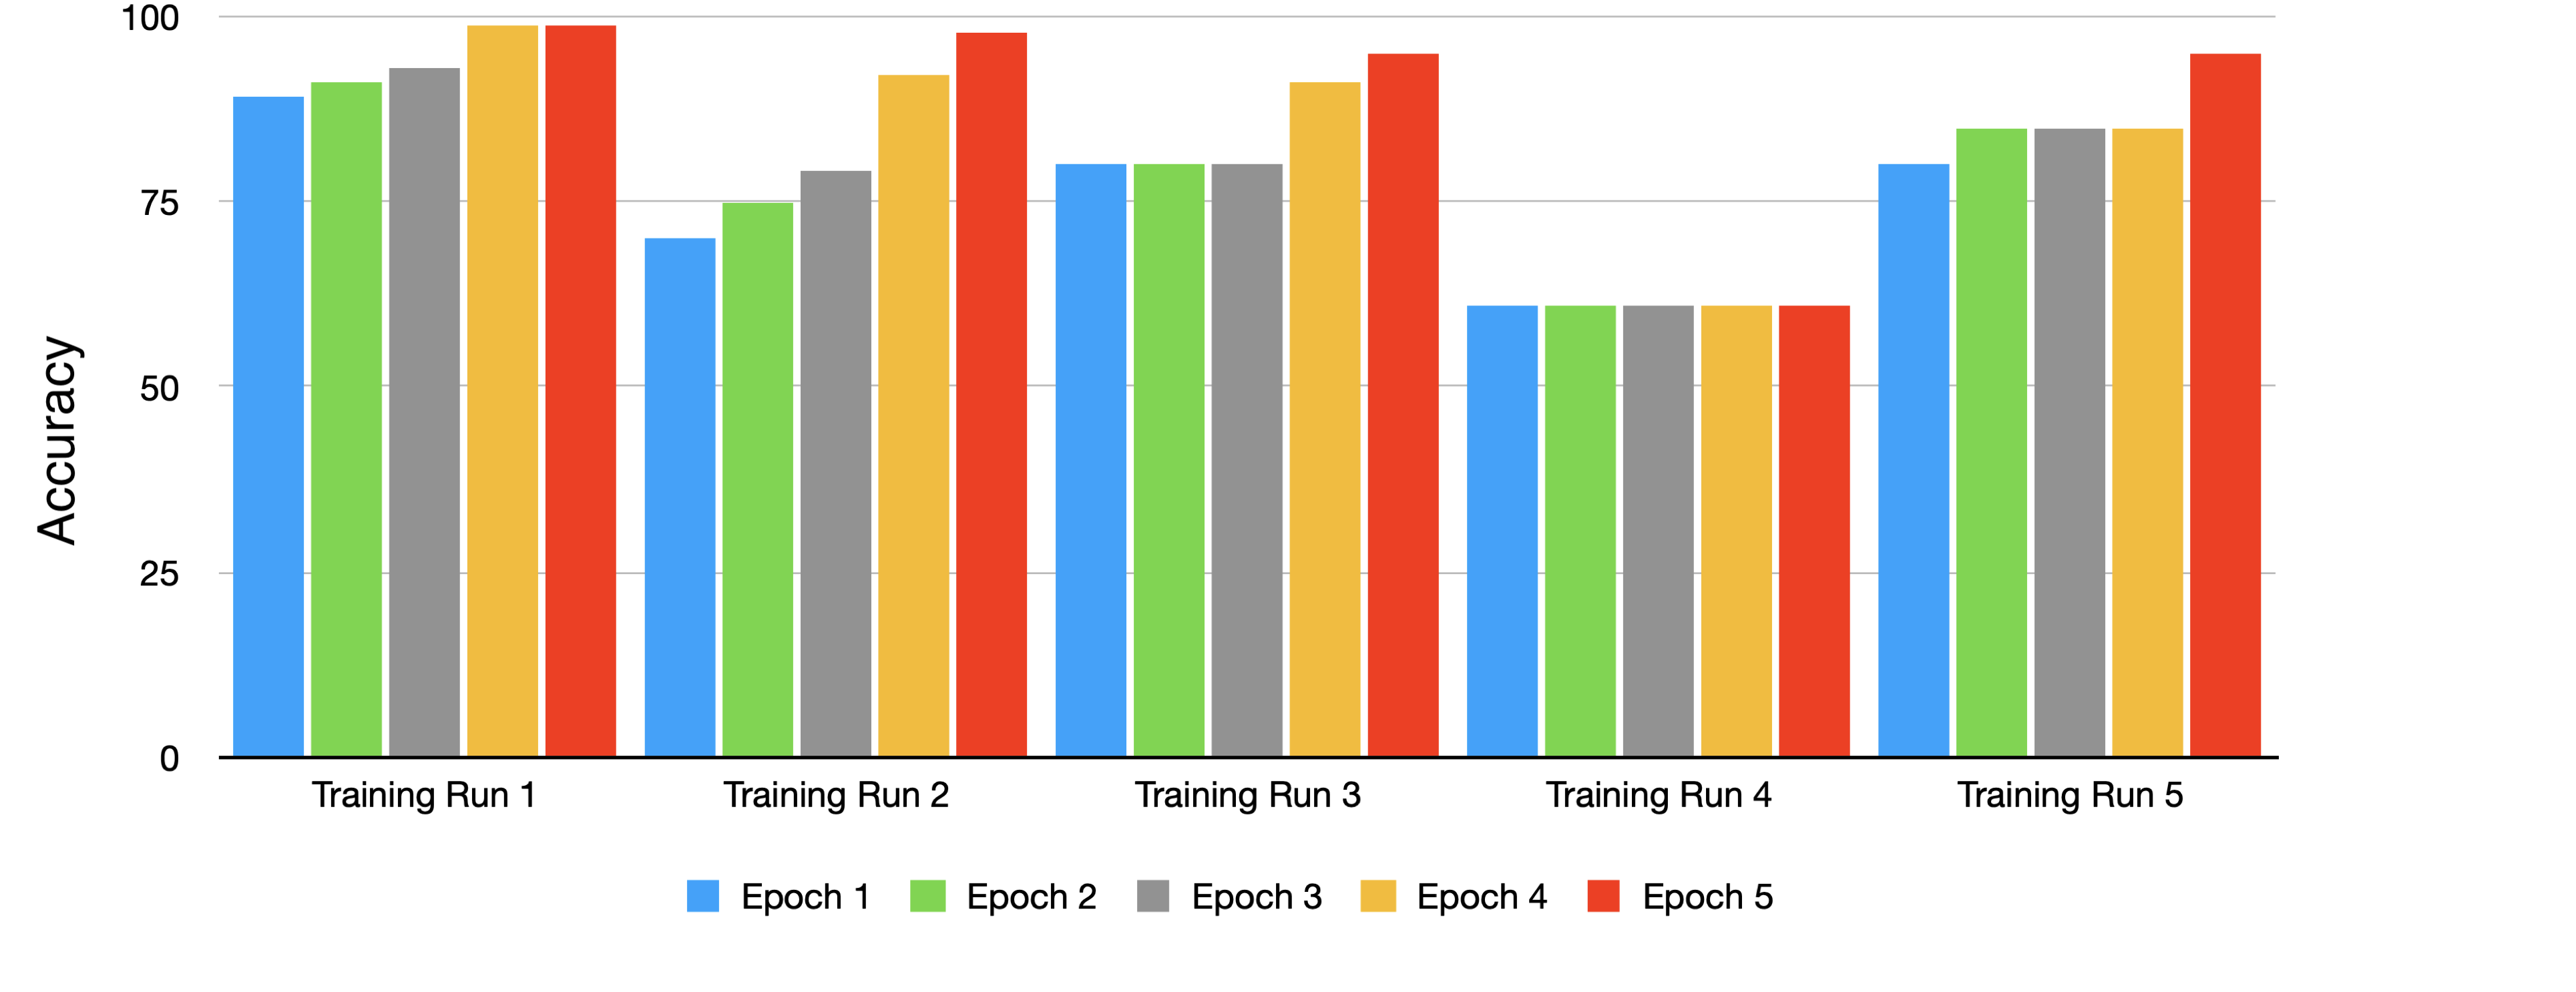
\includegraphics[height = 3.5 cm]{images/training_fig1.png}
        \label{fig:f1}}
        \subfloat{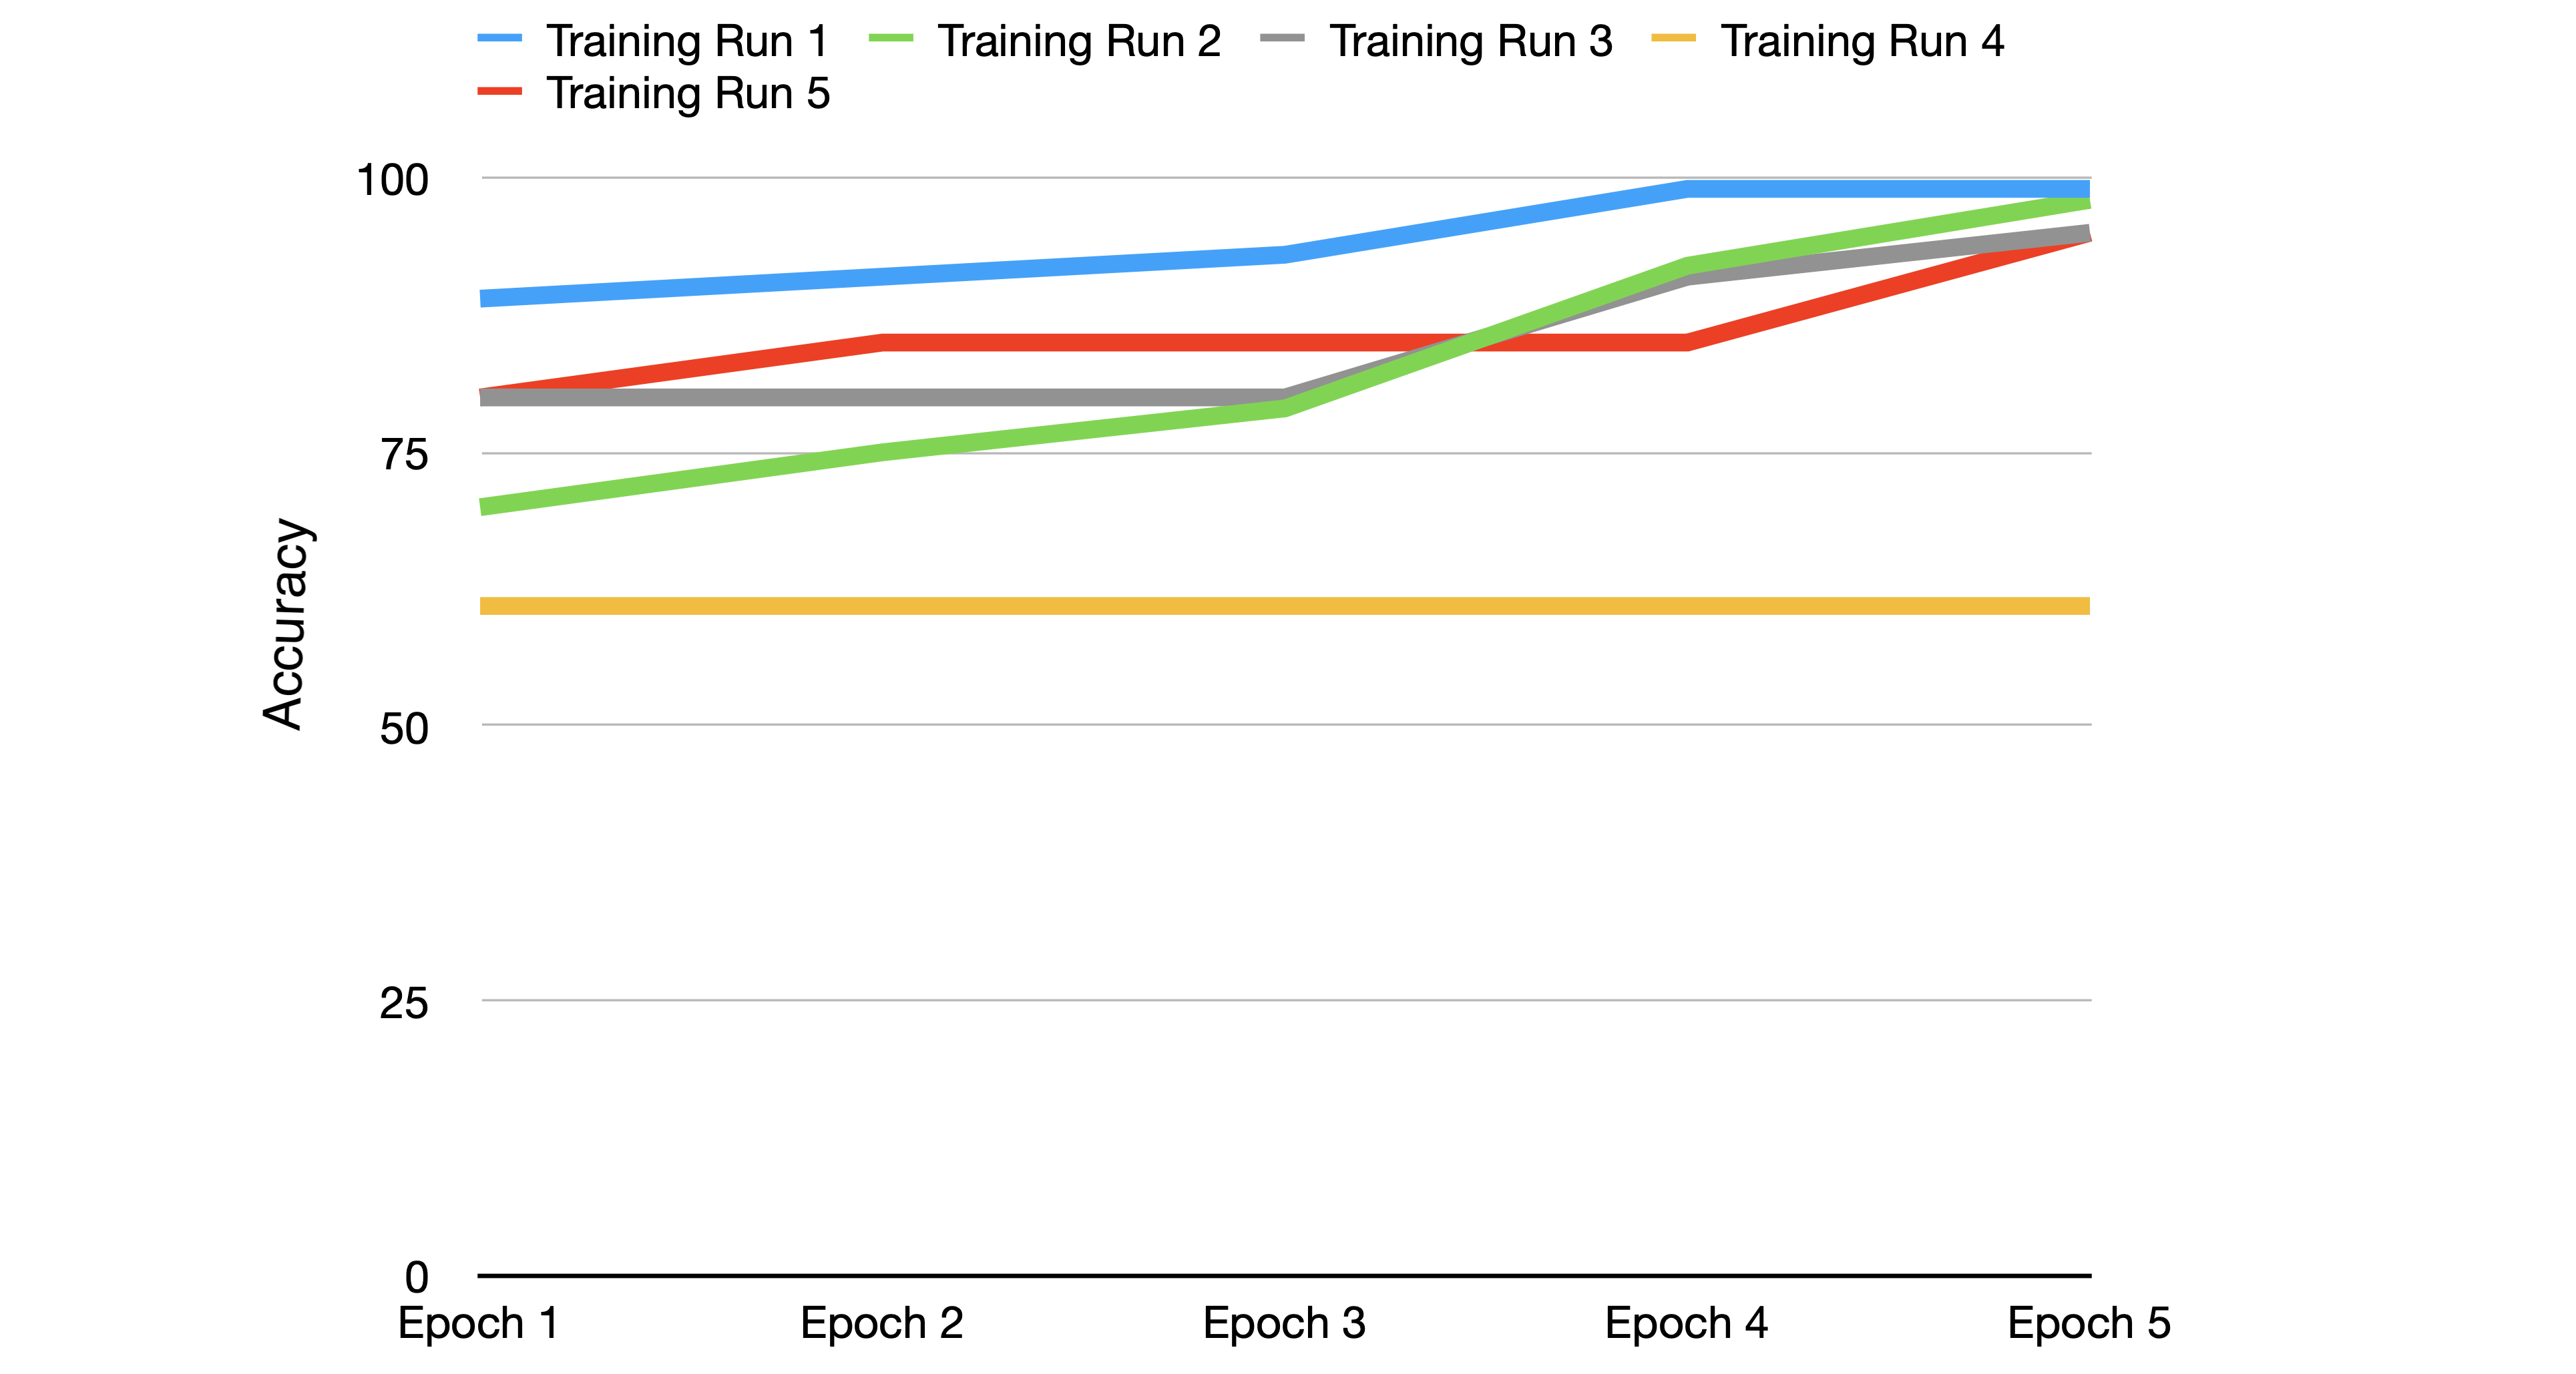
\includegraphics[height = 4 cm]{images/training_fig2.png}
        \label{fig:f2}}
        % \caption{Expanded view of trained and quantized Squeezenet (image was divided}
        \label{netron_sqnet}
    \end{figure}
\end{frame}
\begin{frame}{Inference Performance of Said Model}
    \begin{figure}
        \centering
        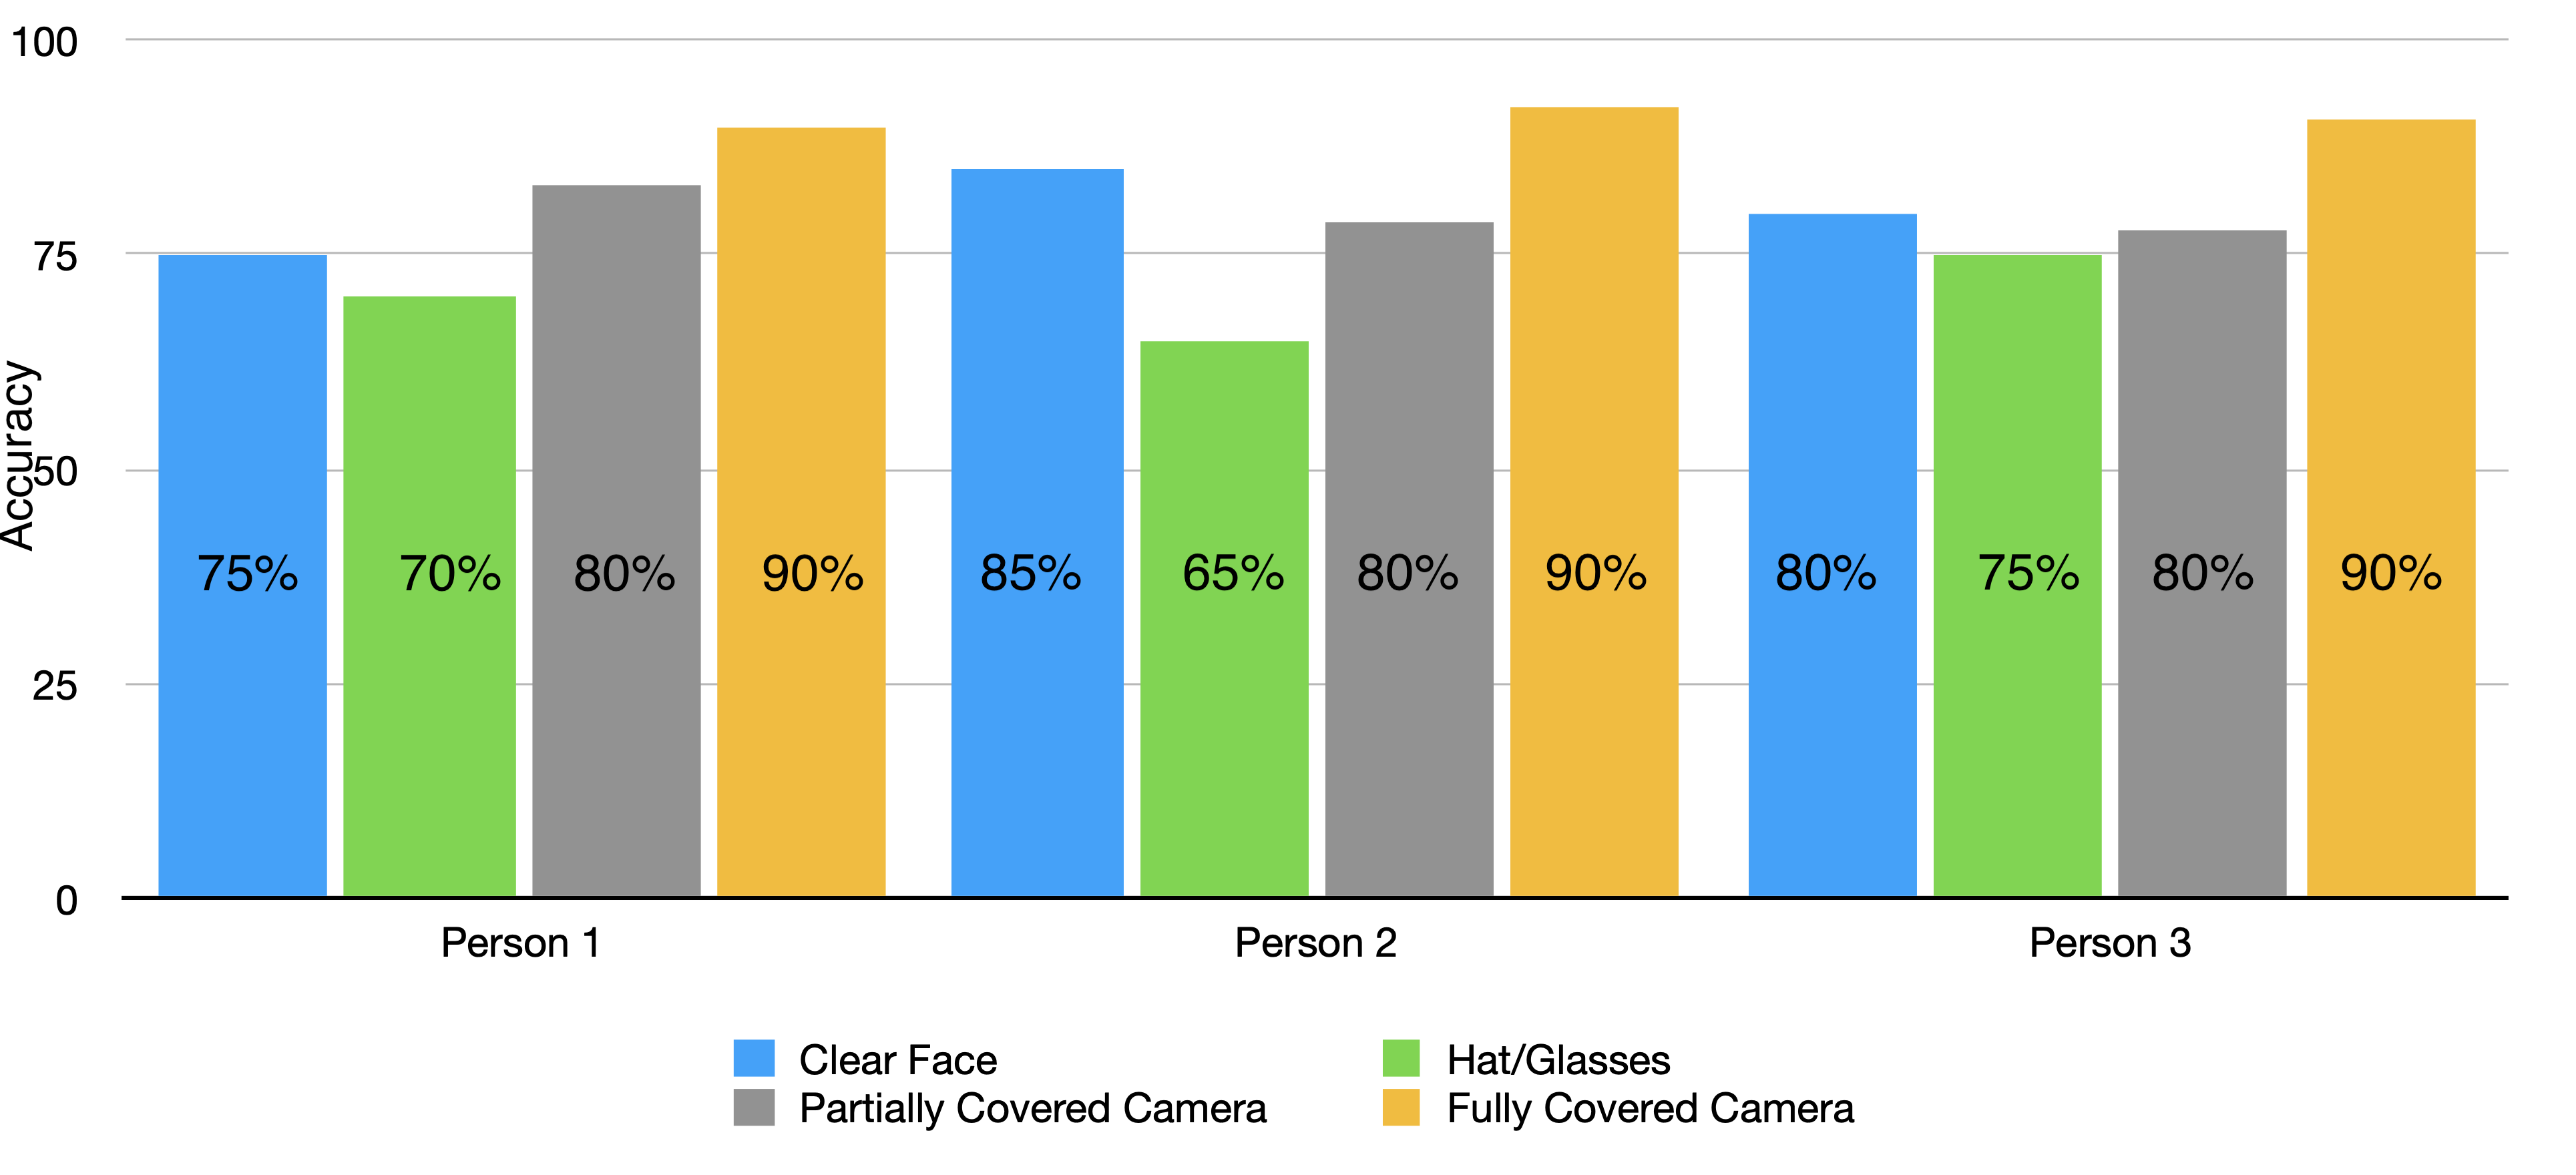
\includegraphics[height = 5 cm]{images/inference_long_test.png}
        \caption{Real-Life Test}
        \label{fig:my_label}
    \end{figure}
\end{frame}

\section{5. Future work}
\begin{frame}{5. Future work}
\begin{itemize}
    \item This thesis demonstrated the possibility of creating accurate, very small-size ML face-recognition models
    \item Proof-of-Concept in a local interpreter
    \item Implementing Face Detection on an embedded device is the next big step
    \item Automating model training is the other big topic to look into
\end{itemize}
\end{frame}

\begin{frame}{The Future of TinyFace}
    \begin{itemize}
        \item Converting TF-Lite Model into compiled C/C++ code
        \item Deploying above code as embedded-board-specific code modules
        \item Building an app to leverage above ML-modules
    \end{itemize}
\end{frame}

\begin{frame}{BSc. Thesis Summary}
    \begin{itemize}
        \item \textbf{Topic}: Machine Learning and Embedded ML
        \begin{itemize}
            \item Dataset Compilation and Processing
            \item Getting to know \& Designing Model Architectures
            \item Training said Models
        \end{itemize}
        \item \textbf{Project 1}: Model Design and Training
        \begin{itemize}
            \item Implemented several ML Models from Research Literature
            \item Trained and Evaluated Performance of said Models
            \item Compared Accuracy using Dataset Pictures and Trained Size
        \end{itemize}
        \item \textbf{Project 2}: Model Performance Evaluation and Benchmark Application
        \begin{itemize}
            \item Built demo-ed Interpreter App 
            \item Evaluated Real-World Performance
        \end{itemize}
    \end{itemize}

    \hspace{}
    \centering
    \item Thank you.
    \centering
\end{frame}

\begin{frame}
    \frametitle{References}
    \footnotesize{
    \begin{thebibliography}{99} 
        \bibitem[1]{tinyml_book} TinyML: Machine Learning with TensorFlow Lite on Arduino and Ultra-Low-Power Microcontrollers
        \newblock Daniel Situnayake and Pete Warden (2020)
        
        \bibitem[2]{lfwild_site} Labelled Faces in the Wild Dataset
        \newblock \hyperlink{Source}{http://vis-www.cs.umass.edu/lfw/}
        
        \bibitem[3]{alignedfaces_site} Aligned Faces Dataset
        \newblock \hyperlink{Source}{http://www.cslab.openu.ac.il/download/wolftau/aligned_images_DB.tar.gz}
        
        \bibitem[4]{ytfaces_site} YouTube Faces dataset 
        \newblock \hyperlink{Source}{https://www.cs.tau.ac.il/~wolf/ytfaces/}
        
        \bibitem[5]{tiny_darknet} Tiny Darknet
        \newblock \hyperlink{Source}{https://pjreddie.com/darknet/tiny-darknet/}
        
        \bibitem[6]{lenet_paper} Backpropagation Applied to Handwritten Zip Code Recognition
        \newblock LeCun, Y. and Boser, B. and Denker, J. S. and Henderson, D. (1989)
        
        \bibitem[7]{vgg_paper} Very Deep Convolutional Networks for Large-Scale Image Recognition
        \newblock Karen Simonyan and Andrew Zisserman (2015)
        \hyperlink{Source}{https://arxiv.org/pdf/1409.1556.pdf}

    \end{thebibliography}
    }
\end{frame}

%-----------------------------------------------------------------------------------
\end{document} 

% \begin{frame}
% \frametitle{Paragraphs of Text}
% Sed iaculis dapibus gravida. Morbi sed tortor erat, nec interdum arcu. Sed id lorem lectus. Quisque viverra augue id sem ornare non aliquam nibh tristique. Aenean in ligula nisl. Nulla sed tellus ipsum. Donec vestibulum ligula non lorem vulputate fermentum accumsan neque mollis.\\~\\

% Sed diam enim, sagittis nec condimentum sit amet, ullamcorper sit amet libero. Aliquam vel dui orci, a porta odio. Nullam id suscipit ipsum. Aenean lobortis commodo sem, ut commodo leo gravida vitae. Pellentesque vehicula ante iaculis arcu pretium rutrum eget sit amet purus. Integer ornare nulla quis neque ultrices lobortis. Vestibulum ultrices tincidunt libero, quis commodo erat ullamcorper id.
% \end{frame}

% %------------------------------------------------

% \begin{frame}
% \frametitle{Bullet Points}
% \begin{itemize}
% \item Lorem ipsum dolor sit amet, consectetur adipiscing elit
% \item Aliquam blandit faucibus nisi, sit amet dapibus enim tempus eu
% \item Nulla commodo, erat quis gravida posuere, elit lacus lobortis est, quis porttitor odio mauris at libero
% \item Nam cursus est eget velit posuere pellentesque
% \item Vestibulum faucibus velit a augue condimentum quis convallis nulla gravida
% \end{itemize}
% \end{frame}

% %------------------------------------------------

% \begin{frame}
% \frametitle{Blocks of Highlighted Text}
% \begin{block}{Block 1}
% Lorem ipsum dolor sit amet, consectetur adipiscing elit. Integer lectus nisl, ultricies in feugiat rutrum, porttitor sit amet augue. Aliquam ut tortor mauris. Sed volutpat ante purus, quis accumsan dolor.
% \end{block}

% \begin{block}{Block 2}
% Pellentesque sed tellus purus. Class aptent taciti sociosqu ad litora torquent per conubia nostra, per inceptos himenaeos. Vestibulum quis magna at risus dictum tempor eu vitae velit.
% \end{block}

% \begin{block}{Block 3}
% Suspendisse tincidunt sagittis gravida. Curabitur condimentum, enim sed venenatis rutrum, ipsum neque consectetur orci, sed blandit justo nisi ac lacus.
% \end{block}
% \end{frame}

% %------------------------------------------------

% \begin{frame}
% \frametitle{Multiple Columns}
% \begin{columns}[c] % The "c" option specifies centered vertical alignment while the "t" option is used for top vertical alignment

% \column{.45\textwidth} % Left column and width
% \textbf{Heading}
% \begin{enumerate}
% \item Statement
% \item Explanation
% \item Example
% \end{enumerate}

% \column{.5\textwidth} % Right column and width
% Lorem ipsum dolor sit amet, consectetur adipiscing elit. Integer lectus nisl, ultricies in feugiat rutrum, porttitor sit amet augue. Aliquam ut tortor mauris. Sed volutpat ante purus, quis accumsan dolor.

% \end{columns}
% \end{frame}

% \begin{frame}
% \frametitle{Table}
% \begin{table}
% \begin{tabular}{l l l}
% \toprule
% \textbf{Treatments} & \textbf{Response 1} & \textbf{Response 2}\\
% \midrule
% Treatment 1 & 0.0003262 & 0.562 \\
% Treatment 2 & 0.0015681 & 0.910 \\
% Treatment 3 & 0.0009271 & 0.296 \\
% \bottomrule
% \end{tabular}
% \caption{Table caption}
% \end{table}
% \end{frame}

% %------------------------------------------------

% \begin{frame}
% \frametitle{Theorem}
% \begin{theorem}[Mass--energy equivalence]
% $E = mc^2$
% \end{theorem}
% \end{frame}

% %------------------------------------------------

% \begin{frame}[fragile] % Need to use the fragile option when verbatim is used in the slide
% \frametitle{Verbatim}
% \begin{example}[Theorem Slide Code]
% \begin{verbatim}
% \begin{frame}
% \frametitle{Theorem}
% \begin{theorem}[Mass--energy equivalence]
% $E = mc^2$
% \end{theorem}
% \end{frame}\end{verbatim}
% \end{example}
% \end{frame}

% %------------------------------------------------

% \begin{frame}
% \frametitle{Figure}
% Uncomment the code on this slide to include your own image from the same directory as the template .TeX file.
% %\begin{figure}
% %\includegraphics[width=0.8\linewidth]{test}
% %\end{figure}
% \end{frame}

% %------------------------------------------------

% \begin{frame}[fragile] % Need to use the fragile option when verbatim is used in the slide
% \frametitle{Citation}
% An example of the \verb|\cite| command to cite within the presentation:\\~

% This statement requires citation \cite{p1}.
% \end{frame}

% %------------------------------------------------